%----------------------------------------------------------------------------
%	   PAQUETES
%----------------------------------------------------------------------------

	\documentclass[twoside]{article}

	\usepackage[sc]{mathpazo} 
	\usepackage[spanish, es-tabla]{babel}
	\usepackage[utf8]{inputenc}

	\usepackage[hmarginratio=1:1,top=32mm,columnsep=20pt]{geometry} % Document margins
	\usepackage{multicol} % Used for the two-column layout of the document
	\usepackage[hang, small,labelfont=bf,up,textfont=it,up]{caption} % Custom captions under/above floats in tables or figures
	\usepackage{mathtools}
	\usepackage{float} % Required for tables and figures in the multi-column environment - [H] needed
	\usepackage{hyperref} % For hyperlinks in the PDF with labels

	\usepackage{abstract} % Allows abstract customization
	\renewcommand{\abstractnamefont}{\normalfont\bfseries} % Set the "Abstract" text to bold
	\renewcommand{\abstracttextfont}{\normalfont\small\itshape} % Set the abstract itself to small italic text

	\usepackage{titlesec} % Allows customization of titles

	\titleformat{\section}[block]{\large\scshape\centering}{\thesection.}{1em}{} % Change the look of the section titles
	\titleformat{\subsection}[block]{\large\centering}{\thesubsection.}{1em}{} % Change the look of the section titles

	\usepackage{fancyhdr} % Headers and footers
	\pagestyle{fancy} % All pages have headers and footers
	\fancyhead{} % Blank out the default header
	\fancyfoot{} % Blank out the default footer
	\fancyhead[C]{Resonador óptico% based on TRACS 
	\hspace{4pt} $\bullet$ \hspace{4pt} Noviembre 2018 } % Custom header text
	\fancyfoot[RO,LE]{\thepage} % Custom footer text

%----------------------------------------------------------------------------
%	   TITLE SECTION
%----------------------------------------------------------------------------

	\title{
		\vspace{-15mm}
		\fontsize{28pt}{10pt}
		\selectfont\textbf{Simulación de las Vibraciones de un Resonador Óptico Confocal}% Article title
	}

	\author{
		\large
		\textsc{Jaime D\'iez Gonz\'alez-Pardo}\\[4mm]
		\fontsize{28pt}{10pt} Universidad de Cantabria \\ % Your institution
		%\thanks{A thank you or further information}\\[2mm] % Your name
		\normalsize Fotónica \\ 
		%\normalsize{Compañeros:} \textsc{NOMBRE COMPANEROS }\\%\normalsize \href{mailto:john@smith.com}{john@smith.com} % Your email address
		%\vspace{5mm}
	}

	\date{ \today }

%----------------------------------------------------------------------------
%       DOCUMENT
%----------------------------------------------------------------------------

	\begin{document}


		\maketitle % Insert title


		\thispagestyle{fancy} % All pages have headers and footers

	%----------------------------------------------------------------------------
	%	  ABSTRACT
	%----------------------------------------------------------------------------

		\begin{abstract}

			\noindent% Dummy abstract text

				Se ha simulado un resonador óptico confocal formado por dos espejos circulares con curvatura en el que con cada reflexión se produce un movimiento aleatorio en la inclinación de ambos espejos. Se ha comparado el campo medio obtenido de 20 simulaciones con el movimiento aleatorio de los espejos, con el campo obtenido con los espejos fijos, obteniendo una relacion de sus picos máximos de $\frac {Max_o}{\overline{Max}} = 0.66$ para el espejo 1 y $\frac{Max_o}{\overline{Max}} = 0.36$ para el espejo 2.

		\end{abstract}

	%----------------------------------------------------------------------------
	%	  ARTICLE CONTENTS
	%----------------------------------------------------------------------------

		\begin{multicols}{2} % Two-column layout throughout the main article text

			\section{Introducción} % Scope of the project = rad effects + minimization
								 
				Un resonador óptico es un dispositivo formado por una serie de espejos que permite confinar los rayos ópticos consiguiendo así amplificar el campo. Existen diferentes configuraciones de resonadores según la disposición y forma de los espejos.

				El resonador confocal es un tipo de resonador formado por dos espejos dispuestos de tal forma que ambos espejos estén situados en la focal del otro, para ello, ambos espejos han de tener misma focal. De esta forma se consigue que ambos espejos se encuentren en el espacio de Fourier del otro, siendo el campo en uno de los espejos la transformada de Fourier del campo en el otro espejo.

				\begin{figure}[H]
					\centering
					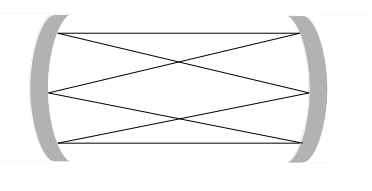
\includegraphics[scale=0.5]{ResonadorConfocal.png}
					\caption{\label{Img:Resonador}Esquema del trazado de los rayos ópticos en un resonador confocal.}
				\end{figure}

				Sin embargo, uno de los grandes problemas de los resonadores ópticos es la alineación de los espejos, pues es impotante conseguir que los espejos están perfectamente centradosy colocados de tal manera que se consiga el fenómeno de confinamiento deseado. Para ello los espejos en los resonadores suelen estar bien fijos y aislados para evitar cualquier movimiento que pueda descolocarlos.

				En este informe se ha tratado de estudiar las posibles perdidas producidas por pequeñas vibraciones de los espejos comparando los resultados que se obtienen con los resultados que se obtendrían con los espejos perfectamente fijos sin movimientos. Para ello se han simulado ambas situaciones.

			\section{Desarrollo Experimental}

				El estudio de los resonadores se ha realizado mediante la simulación de estos a partir del código \cite{Resonador} escrito por el alumno en el lenguaje Python. Para ello se ha trabajado con el problema como un sistema lineal en el que cada rebote es equivalente a la transformada de Fourier del producto del campo que llega al espejo por el propio espejo.

				El código utilizado contiene una clase Espejo que permite crear los espejos del resonador teniendo en cuenta el tamaño del campo, el tamaño del espejo, forma del espejo, curvatura e inclinación. Para este estudio se ha simulado un campo de 600 por 600 en un resonador formado por dos espejos iguales de forma circular con diámetro 120 y curvatura 0.01. Los espejos han partido perfectamente alineados sin inclinación, pero se han ido moviendo de manera aleatoria en un rango de $[-0.25^o, 0.25^o]$ en cada una de las reflexiones tratando de imitar el posible movimiento aleatorio debido a vibraciones. En el apéndice \ref{appen:Espejo} se muestra como se ha obtenido la matriz Espejo.

				Al tratarse de un movimiento aleatorio de los espejos, se ha realizado la simulación de resonador 20 veces con la misma configuración y el mismo número de reflexiones para obtener el campo medio y comparar este con el obtenido con los espejos fijos.

			\section{Resultados}

				Se ha simulado un resonador óptico confocal en un campo de 600 por 600, formado por dos espejos circulares de diámetro 120 y una curvatura de 0.01. En la rimulación se han realizado 25 reflexiones en cada espejo hasta obtener el campo.

				Se ha realizado una simulación manteniendo los espejos fijos y 20 simulaciones realizando un movimiento aleatorio de los dos espejos en un rango de $[-0.25^o , 0.25^o]$, obteniendo un campo medio a partir de los campos de las 20 simulaciones.

				En la Figura \ref{Img:Espejo1} se muestran los campos obtenidos en el espejo 1 tras realizar las simulaciones. Las dos gráficas de arriba corresponden al campo sin movimiento de los espejos y las dos de abajo al campo medio obtenido del movimiento de los espejos.

					\begin{figure}[H]
						\centering
						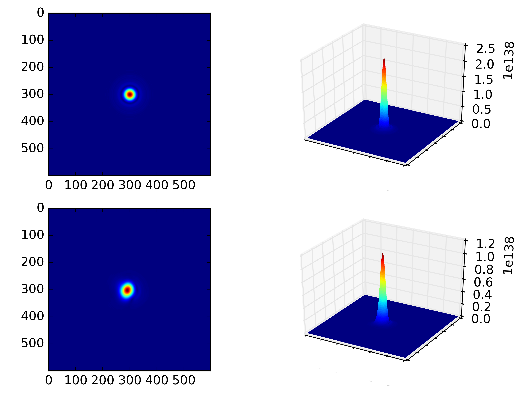
\includegraphics[scale=0.25]{FiguraEspejo1.png}
						\caption{\label{Img:Espejo1}Campos obtenidos en el espejo 1 tras realizar las simulaciones. Las dos gráficas de arriba corresponden al campo sin movimiento de los espejos y las dos de abajo al campo medio obtenido del movimiento de los espejos.}
					\end{figure}

				En la Figura \ref{Img:Espejo2} se muestran los campos obtenidos en el espejo 2 tras realizar las simulaciones. Las dos gráficas de arriba corresponden al campo sin movimiento de los espejos y las dos de abajo al campo medio obtenido del movimiento de los espejos.

					\begin{figure}[H]
						\centering
						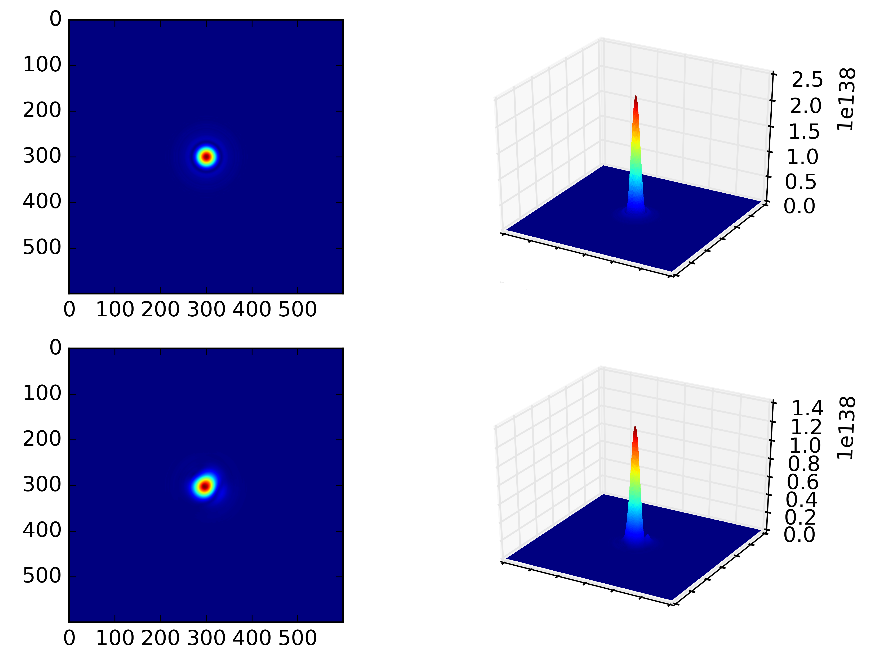
\includegraphics[scale=0.25]{FiguraEspejo2.png}
						\caption{\label{Img:Espejo2}Campos obtenidos en el espejo 2 tras realizar las simulaciones. Las dos gráficas de arriba corresponden al campo sin movimiento de los espejos y las dos de abajo al campo medio obtenido del movimiento de los espejos.}
					\end{figure}

				En la Tabla \ref{Tab:Maximum} se muestran los valores del maximo del campo obtenido para el espejo fijo $Max_0$ y de la media de los campos con movimiento aleatorio $\overline{Max}$, para los dos espejos.

					\begin{table}[H]
						\centering
						\begin{tabular}{c | c c }
							\hline
							\centering
								 & Espejo 1 & Espejo 2 \\ \hline
								$Max_0 \cdot 10^{135}$ & 2.93 & 846.16 \\
								$\overline{Max} \cdot 10^{135}$ & 1.95 & 2346.55 \\ \hline

						\end{tabular}
						\caption{\label{Tab:Maximum}Maximo del campo obtenido para el espejo fijo $Max_0$ y de la media de los campos con movimiento aleatorio $\overline{Max}$, para los dos espejos.}
					\end{table}
			
				A partir de estos valores se puede obtener una relaci\'on entre los valores obtenidos con los espejos fijos y con un movimiento de estos aleatroio.

					\begin{equation}
						\textrm{Espejo 1} \rightarrow \frac {Max_o}{\overline{Max}} = 0.66
					\end{equation}

					\begin{equation}
						\textrm{Espejo 2} \rightarrow \frac {Max_o}{\overline{Max}} = 0.36
					\end{equation}

			\section{Discusión}

				Se han obtenido las relaciones entre los picos máximos de los campos en los espejos con y sin movimiento aleatorio. En las Figuras \ref{Img:Espejo1} y \ref{Img:Espejo2} se observa como los campos con y sin movimiento aleatorio mantienen una forma muy parecida para ambos espejos, manteniendo un único pico estrecho circular. Sin embargo, sí se pueden apreciar en las proyecciones en dos dimensiones que para el caso de movimientos aleatorios el pico pierde la forma circular observando pequeñas deformaciones en la base.

				No obstante, la mayor diferencia se aprecia al comparar los valores de los picos, obteniendo unas perdidas del $34\%$ para el espejo 1 y del $64\%$ para el espejo 2 para el caso del movimiento aleatorio de los espejos.

			\section{Conclusiones}

				Se ha logrado observar la gran importancia que tiene en los resonadores ópticos confocales el conseguir mantener los espejos fijos con el alineamiento preciso, tratando de absorver todos los movimientos, pues se ha obtenido que para movimientos aleatorios de los espejos en un rango de $[-0.25^o, 0.25^o]$ se producen pérdidas de entorno al $50\%$.

		\end{multicols}

	%----------------------------------------------------------------------------
	%     APPENDIX
	%----------------------------------------------------------------------------

		%\newpage

		    \appendix

		    	\section{Obtención del Espejo}
		    		\label{appen:Espejo}

					Para  $(\sqrt{k^2+j^2}=r_{k,j}) < R$:

						\begin{equation}
							Espejo_{k, j} = 1 \cdot e^{i\cdot crv \cdot r_{k,j}} \cdot e^{i\cdot (tip\cdot r_k + tilt \cdot r_j)}
						\end{equation}
						
					Para $(\sqrt{k^2+j^2}=r_{k,j}) = R$:

						\begin{equation}
							Espejo_{k,j} = 0.5 \cdot e^{i\cdot crv \cdot r_{k,j}} \cdot e^{i\cdot (tip\cdot r_k + tilt \cdot r_j)}
							\label{eq:Espejo}
						\end{equation}	

					Siendo $(k, j)$ las coordenadas $(x, y)$ de la matriz, $r_{k, j}$ el radio de esas coordenadas respecto al centro de la matriz, $R$ el radio del espejo, $crv$ la curvatura, $tip$ la inclinación respecto al eje $X$ y $tilt$ la inclinación respecto al eje $Y$.
		    		
	%----------------------------------------------------------------------------
	%     BIBLIOGRAPHY
	%----------------------------------------------------------------------------

		\bibliographystyle{unsrt}
		\bibliography{biblio}

	\end{document}

%----------------------------------------------------------------------------
%            TEMPLATES
%----------------------------------------------------------------------------

	%----------------------------------------------------------------------------
	%            how to insert an image
	%----------------------------------------------------------------------------

	%	\begin{figure}[H]
	%		\centering
	%		\includegraphics[scale= ]{nombre de la imagen.jpg}
	%		\caption{\label{Img:widgets}el pie de pagina que le quieras 	poner a la imagen}
	%	\end{figure}
	 
	%----------------------------------------------------------------------------
	%            how to insert a table
	%----------------------------------------------------------------------------

	%	\begin{table}[H]
	%		\centering
	%		\begin{tabular}{|c|c|c|c|}
	%			\hline
	%			\centering
	%				Altura(h) & Distancia (d) & Elaboracion (e) & Longitud (l) \\
	%				($\pm0.5$ mm) & ($\pm0.5$ mm) & ($\pm0.5$ mm) & ($\pm0.5$ mm) \\ \hline
	%				 &  &  &  \\ \hline
	%				 &  &  &  \\ \hline
	%				 &  &  &  \\ \hline
	%				 &  &  &  \\ \hline
	%				 &  &  &  \\ \hline
	%		         &  &  &  \\ \hline
	%		\end{tabular}
	%		\caption{\label{Tab:widgets}pie de pagina que le quieras poner}
	%	\end{table}

	%----------------------------------------------------------------------------
	%             How to remove the label in equactions
	%----------------------------------------------------------------------------

	%	\begin{equation*}
	%		
	%	\end{equation*}

	%----------------------------------------------------------------------------
	%              How to set bibliography
	%----------------------------------------------------------------------------

	%\bibliographystyle{unsrt}
	%\bibliography{biblio}
	%
	%Then you have to set a .bib document such as the next template
	%
	%	@book{nickname,
	%	author = {},
	%	title = {},
	%	edition = {},
	%	year = {},
	%	volume = {},
	%	ISBN = {}
	%	}
	%
	%	@ARTICLE{nickname,
	%	author = {},
	%	title = {},
	%	year = {},
	%	volume = {},
	%	}

%----------------------------------------------------------------------------
%              END
%----------------------------------------------------------------------------